\section{MVE}\label{sec:mve}
%======================================================================================
%
Um dos algoritmos utilizados para a técnica de reconstrução densa é o MVE -- {\it Multi-View  Environment}, feito por Simon Fuhrmann, Fabian Langguth e Michael Goesele. Este algoritmo utiliza fotos e produz uma malha triangular superficial como resultado. Diferente das reconstruções baseadas nas geometria das imagens, o MVE é focado na reconstrução multi-escala, um quesito importante na reconstrução de esculturas e acervo cultural. Portanto, com esta técnica é possível reconstruir grandes volumes de dados, contendo regiões detalhadas em alta resolução, em comparação com o resto da cena. O sistema ainda possui uma interface gráfica para o uma reconstrução baseada no SfM, amigável ao usuário (UMVE), onde permite a visualização e inspeção das imagens, mapas de profundidade e renderizar cenas e malhas 3D.

Sua base de operação é basicamente:

\begin{enumerate}
\item{Estrutura da formação -- {\it Structure-from-Motion} (SfM)}

\begin{itemize}
\item{
Reconstrói os parâmetros da câmera (posição e orientação) e seus dados de calibração (distância focal e distorção radial),
encontrando correspondências esparsas mas estáveis entre as imagens. (Já foi abordado em outra seção deste manuscrito).
}
\end{itemize}

\item{Múltiplas visões estéreo -- {\it Multi-View Stereo} (MVS)}
\begin{itemize}
\item{
Utiliza a posição estimada das câmeras, encontrando as correspondências visuais nas imagens. Estas correspondências são trianguladas, produzindo a informação 3D, e,
consequentemente a reconstrução 3D densa.
} 
\end{itemize}
\item{Reconstrução de superfícies -- {Surface Reconstruction}}
\begin{itemize}
\item{
Tem como entrada uma densa nuvem de pontos, ou mapas de profundidade individuais. Produz uma malha superficial globalmente consistente.
}
\end{itemize}
\end{enumerate}

Como não existem muitas opções para algoritmos de SfM, o MVE permite a utilização de {\it softwares} externos como o {\it Bundler} ou o prório {\it VisualSfM}.

Uma vez com o passo do SfM feito, partimos para o MVS. Com os parâmetros de câmera conhecidos, a reconstrução densa geométrica é feita. Existem diversos algoritmos para a reconstrução densa, o MVE no caso, utiliza um algoritmo próprio, feito por um de seus criadores, Michael Goesele ({\it Multi-View Stereo for Community Photo Collections approach}), que reconstrói um mapa de profundidade para cada foto. 

Embora abordagens baseadas em mapeamentos de profundidade produzirem uma grande quantidade de redundância, (isso se dá por causa das inúmeras fotos que são sobrepostas e possuírem partes similares da mesma cena), este algoritmo é altamente escalável para grandes cenas, pois apenas um pequeno conjunto de fotos vizinhas é necessário para a reconstrução. Outra vantagem da utilização dos mapas de profundidade como representação intermediária é que a geometria é parametrizada em seu domínio natural, e os dados por foto (como a cor, por exemplo) estão diretamente acessíveis nas imagens.

A redundância excessiva nos mapas de profundidade pode ser pesado. Não com relação ao armazenamento, mas na questão do processamento computacional exigido nos mapas de profundidade. Porém, esta abordagem foi capaz de produzir uma geometria detalhada e superar o ruído nos mapas de profundidades individuais.

\subsection{Guia de reconstrução com o MVE}

% Capturing photos: A dataset reconstructs best if a few sim-
% ple rules are observed. First, in order to successfully recon-
% struct a surface region, it must be seen from at least five
% Figure 5: The final surface reconstruction with color (left)
% and shaded (right). Notice how even the engraved text is vis-
% ible in the geometry.
% views. This is a requirement of the MVS algorithm to reli-
% ably triangulate any 3D position. Photos should thus be taken
% with a good amount of overlap. Usually, unless the dataset
% becomes really large, more photos will not hurt quality, but
% there is a tradeoff between quality and performance. As a
% rule of thumb, taking twice as many photos as one might
% think is a good idea. In order for triangulation to work, paral-
% lax is required. The camera should be re-positioned for every
% photo. (This is exactly opposite to how panoramas are cap-
% tured, where parallax in the images must be avoided.) This is
% also important for SfM: Triangulating a feature track with in-
% sufficient parallax results in a small triangulation angle and a
% poorly conditioned 3D position. Figure 6 shows some input
% images of our exemplary dataset.

Tirando fotos: Um bom conjunto de dados é gerado se algumas regras simples forem seguidas:

\begin{ìtemize}
\item{Para que o algoritmo do MVS consiga fazer uma triangulação com qualquer posição 3D, o conjunto de dados terá que ter, no mínimo, cinco fotos.}
\item{As fotos devem ser tiradas com uma boa quantidade de sobreposição. A menos que o conjunto de dados se torne muito grande, uma grande quantidade de fotos não prejudicará a qualidade. 
Mas terá uma compensação do sistema, no que diz respeito à qualidade e desempenho.}
\item{Para a triangulação funcionar, é necessário que tenha o efeito de paralaxe \ref{fig:parallax} (Aparente mudança na posição do objeto). Ou seja, é interessante que o conjunto de imagens seja duplicado.}
\item{A câmera deverá ser reposicionada, de preferência.}
\end{itemize}

\begin{figure} [!h]
	\centering
	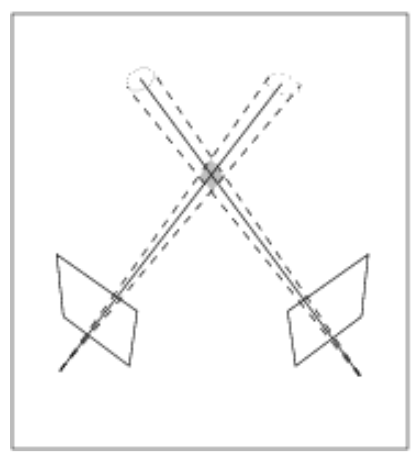
\includegraphics[width=0.45\linewidth]{figs/parallaxA.png}(a)
	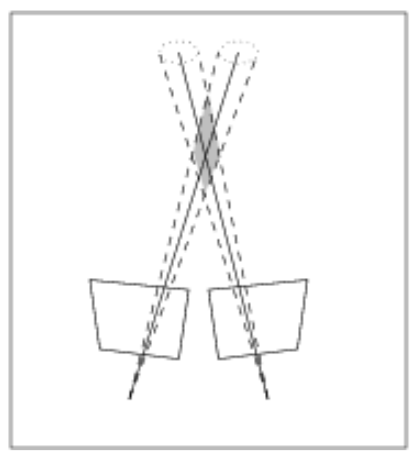
\includegraphics[width=0.45\linewidth]{figs/parallaxB.png}(b)
	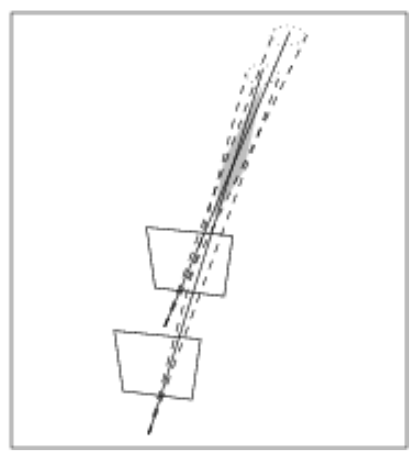
\includegraphics[width=0.45\linewidth]{figs/parallaxC.png}(c)
	\caption{%
	Caso o espaçamento entre as câmeras seja grande, a informação extraída das imagens em comum será menor (a). Se a angulação do efeito de paralaxe seja baixa, terá a mesma informação sobre um ponto em questão (c). Ou seja utilizando ou (a), ou (c). Pode ser que a reconstrução fique incerta. Para que o efeito paralaxe tenha maior proveito das imagens das câmeras, é necessário que as câmeras estejam dispostas como (b), conseguindo extrair uma boa quantidade e qualidade de informações do ponto.
	}
	}\label{fig:parallax}
\end{figure}

% Creating a scene: A view is a container that contains per-
% viewport data (such as images, depth maps and other data).
% A scene is a collection of views, which make up the dataset.
% A new scene is created using either the graphical interface of
% our software, UMVE, or the command line tool makescene.
% Technically, the scene appears as a directory in the file sys-
% tem (with the name of the dataset). It contains another direc-
% tory views/ with all views stored as files with the extension
% .mve. Creating a new scene will solely create the views/
% directory for now. Importing photos will create a .mve file
% for every photo. This process will also import meta informa-
% tion from the images (EXIF tags), which is required to get
% a focal length estimate for every photo. If EXIF tags are not

Criando uma cena: Uma visualização contém dados por exibição (como imagens, mapas de profundidade ou outros dados). Uma cena é uma coleção de visualizações, que constitui um conjunto de dados. Uma nova cena pode ser criada utilizando a interface gráfica UMVE, ou por linha de comando ({\it makescene}). 

Tecnicamente, a cena é criada como um diretório no sistema de arquivos (com o nome do conjunto de dados). Este, por sua vez, contém outro diretório ({\it views}), com todas as visualizações guardadas com uma extensão de arquivos em .MVE.

Criar uma nova cena, criará apenas o diretório ({\it views}) vazio. A importação de fotos criará arquivos .MVE para cada foto. Esse processo importará meta-dados provenienteas das imagens ({\it tags} EXIF), que é necessário para estimar a distância focal para cada foto. Caso estes meta-dados não estejam disponíveis, uma distância focal padrão é assumida pelo sistema, porém se essa distância adotada for uma péssima suposição, com relação ao conjunto de dados utilizado, pode vir a acontecer erros no SfM.

//-----------------------------------------------------------FOTO UMVE AQUI-------------------------------------------------------------//

% SfM reconstruction: The SfM reconstruction can be con-
% figured and started using UMVE, or the command line tool
% sfmrecon. The UI guides through feature detection, pairwise
% matching and incremental SfM. What follows is the SfM re-
% construction starting from an initial pair, and incrementally
% adding views to the reconstruction. Finally, the original im-
% ages are undistorted and stored in the views for the next step.
% Figure 8 shows a rendering of the SfM reconstruction with
% the sparse point cloud and the camera frusta. Note how dense
% the frusta are spaced around the object to achieve a good re-
% construction.

Reconstrução SfM: Pode ser configurada e iniciada usando a interface gráfica UMVE ou por linha de comando ({\it sfmrecon}). A interface guia através da detecção de {\it features}, combinação emparelhada ({\it pairwise matching}) e uso incremental do SfM. Que, por sua vez, a reconstrução SfM começa a partir de um par inicial, e adiciona, de forma incremental, mais vistas à reconstrução.

//---------------------------------------FOTO RECONSTRUÇÃO UMVE---------------------------------------------------------------------//